\section{Resultados}
\subsection{Conversor digital-análogo}

\begin{verbatim}
RESET:
    ; Apuntar Z al inicio de la LUT
    ldi ZH, HIGH(LUT_START<<1)
    ldi ZL, LOW(LUT_START<<1)

	; Apuntar Y al final de la LUT
	ldi YH, HIGH(LUT_END<<1)
	ldi YL, LOW(LUT_END<<1)
\end{verbatim}

\begin{verbatim}
MAIN_LOOP:
    ; Leer siguiente valor de la LUT
    ; y avanzar puntero
    lpm r16, Z+
    out PORTD, r16
    rcall delay

    cp  ZL, YL
    cpc ZH, YH
    ; Si no es el fin, seguir
    brne MAIN_LOOP

    ; Volver al inicio de la tabla
    ldi ZH, HIGH(LUT_START<<1)
    ldi ZL, LOW(LUT_START<<1)
    rjmp MAIN_LOOP
\end{verbatim}

\begin{figure}[H]
  \centering
  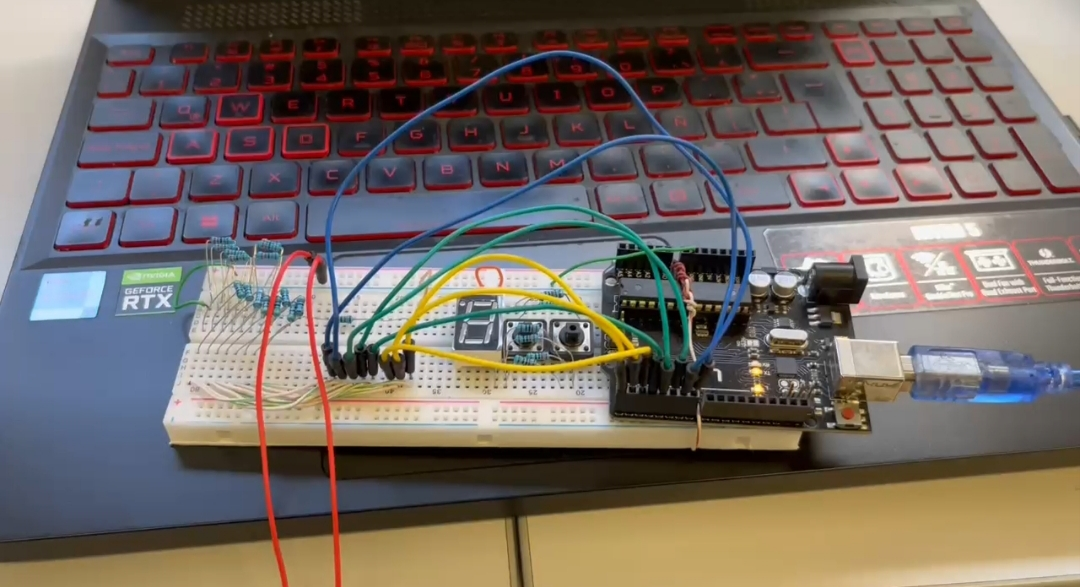
\includegraphics[width=\linewidth]{./Anexos/Resultados/DAC/Circuito.jpg}
  \caption{Circuito final para conversor digital-análogo. Fuente: \cite{LabDrive}.}
  \label{fig:conversor_circuito}
\end{figure}

\begin{figure}[H]
  \centering
  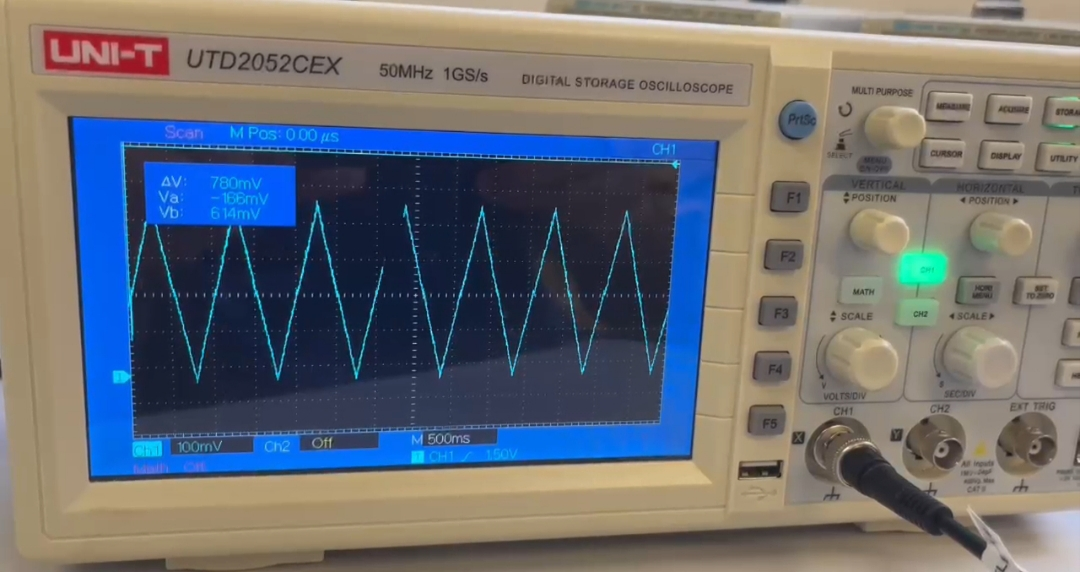
\includegraphics[width=\linewidth]{./Anexos/Resultados/DAC/Ocsiloscopio.jpg}
  \caption{visualización de señal en osciloscopio. Fuente: \cite{LabDrive}.}
  \label{fig:conversor_osciloscopio}
\end{figure}

\subsection{Matriz}

\subsubsection{Mapeado de puertos y pines}
Se mapean los puertos y pines individuales del mismo modo al que se puede apreciar en el anexo \ref{anexo:Look_Up_Table}.

\subsubsection{Encendido de un solo LED}
\begin{verbatim}
ldi ZH, high(ROW_PORTS<<1) 
ldi ZL, low(ROW_PORTS<<1)
add ZL, row adc ZH, r1  
lpm r16, Z ; r16 = row port adress
        
ldi ZH, high(ROW_MASKS<<1) 
ldi ZL, low(ROW_MASKS<<1)
add ZL, row adc ZH, r1
lpm r17, Z ; r18 = row pin mask

; Encender fila
clr ZH mov ZL, r16 
mov r16, r17
rcall CLEAR_BIT

ldi ZH, high(COL_PORTS<<1) 
ldi ZL, low(COL_PORTS<<1)  
add ZL, col adc ZH, r1  
lpm r16, Z ; r16 = column port adress

ldi ZH, high(COL_MASKS<<1) 
ldi ZL, low(COL_MASKS<<1)  
add ZL, col adc ZH, r1  
lpm r17, Z ; r17 = column pin mask

; Encender columna
clr ZH mov ZL, r16 
mov r16, r17
rcall SET_BIT
\end{verbatim}

\subsubsection{Multiplexado y dibujo de cuadros}
\begin{verbatim}
ldi row, 0 RENDER_FRAME_ROW_LOOP:  
ldi r16, 0b00000001 ; Frame mask
lpm r17, Z+

ldi col, 0 RENDER_FRAME_COL_LOOP:
    rcall CLEAR_MATRIX

    push r16
    and r16, r17

    cpi r16, 0 
    breq RENDER_FRAME_SKIP_LED

    rcall TURN_LED
    rcall TEST_DELAY

    RENDER_FRAME_SKIP_LED:
    pop r16
    lsl r16
inc col cpi col, 8 
brlo RENDER_FRAME_COL_LOOP 

inc row cpi row, 8 
brlo RENDER_FRAME_ROW_LOOP
\end{verbatim}

Manejo de cambio de estados utilizando USART para mostrar las diferentes imágenes en la matriz

\begin{verbatim}
USART_RX_ISR:	
    lds r16, UDR0

    ; Apagar pantalla
    cpi r16, '0' 
    breq USART_RX_ISR_CASE_0 

    ; Texto desplazante
    cpi r16, '1' 
    breq USART_RX_ISR_CASE_1 

    ; ...

USART_RX_ISR_CASE_0:
    rcall SET_ANIMATION_START
    ; Disable timer interrupts
    ldi r16, 0b0 sts TIMSK2, r16 
    ; Change state
    ldi r16, 0 mov current_state, r16   
    rjmp USART_RX_ISR_END

USART_RX_ISR_CASE_1:
    rcall SET_ANIMATION_START
    ; Change state
    ldi r16, 1 mov current_state, r16   
    ; Enable timer interrupts
    ldi r16, 0b1 sts TIMSK2, r16 
    rjmp USART_RX_ISR_END

    ; ...
\end{verbatim}

Aparte del manejo del cambio de estado, se implementó una máquina de estados, como la que se puede encontrar en el anexo \ref{anexo:Maquina_de_Estados}.

\begin{verbatim}
MAIN:
    rcall STATE_MACHINE
    rjmp MAIN
\end{verbatim}

Circuito final realizado:

\begin{figure}[H]
  \centering
  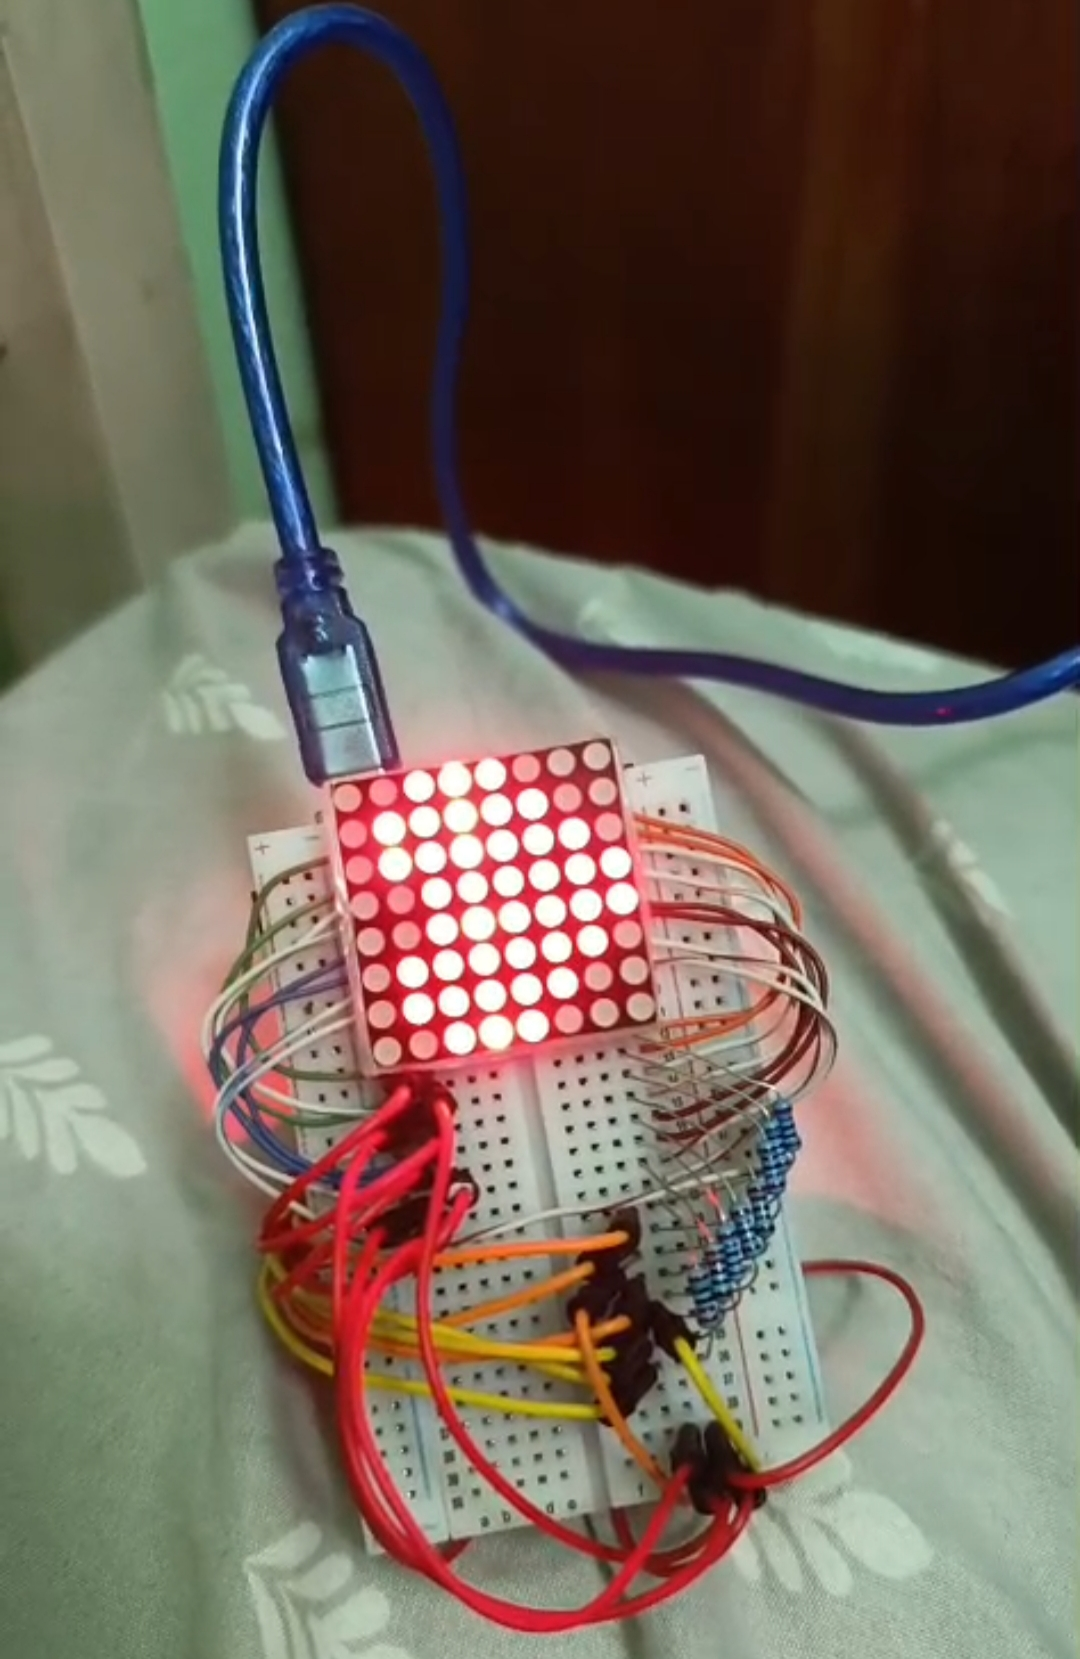
\includegraphics[width=0.7\linewidth]{./Anexos/Resultados/Matriz/Circuito.jpg}
  \caption{Circuito final para Matriz de LEDs. Fuente: \cite{LabDrive}.}
  \label{fig:circuito_matriz}
\end{figure}


\section{Punzonadora}

\subsubsection{Configuración de temporizador variable}
\begin{verbatim}
.macro ENABLE_TIMER_1
; @0 Timer seconds
push r16
mov timer1_ovf_counter, @0
ldi r16, 0b101		 sts TCCR1B, r16
ldi r16, HIGH(49911) sts TCNT1H, r16
ldi r16, LOW(49911)	 sts TCNT1L, r16 
ldi r16, (1<<TOV1)   out TIFR1,  r16 
ldi r16, (1<<TOIE1)  sts TIMSK1, r16 
pop r16
.endmacro
\end{verbatim}


\subsubsection{Manejo de estados}

Control de estados general:
\begin{verbatim}
STATE_MACHINE:
cpi state, 0 breq STATE_MACHINE_STOP
cpi state, 1 breq STATE_MACHINE_ADVANCE
cpi state, 2 breq STATE_MACHINE_WAIT_1
cpi state, 3 breq STATE_MACHINE_PUNCH
cpi state, 4 breq STATE_MACHINE_WAIT_2
cpi state, 5 breq STATE_MACHINE_EXTRACT
rjmp STATE_MACHINE_END
\end{verbatim}

Control de estados individual, cada caso tiene un manejo de tiempos específico dictado por el diagrama de estados mostrado con anterioridad.
\begin{verbatim}
STATE_MACHINE_STOP:
cpi load, 0 breq STOP_LOAD_0
cpi load, 1 breq STOP_LOAD_1
cpi load, 2 breq STOP_LOAD_2
rjmp STATE_MACHINE_STOP_SKIP
\end{verbatim}

\subsubsection{Botones, LEDs,  y debouncing}
Interrupción se descativa sola. Se vuelve a habilitar cuando la máquina de estados llega al final del recorrido:

\begin{verbatim}
INT0_ISR:
    push r16
    in r16, SREG
    push r16 

    DISABLE_BUTTONS
    DISABLE_RX

    ldi state, 1
    ldi r16, 1 
    sts event_pending, r16

    pop r16
    out SREG, r16
    pop r16 
    reti
\end{verbatim}

Temporizador de deboucing para botones de cambio de carga. Timer 2 configurado para un overflow de aproximadamente 1 segundo (usando contador de overflow externo):

\begin{verbatim}
    T2_OVF_ISR:
	push r16 
    in r16, SREG 
	push r16 
	
	inc timer2_ovf_counter
	
	ldi r16, _TIMER2_OVF_COUNT 
    cp r16, timer2_ovf_counter 
    brsh T2_OVF_ISR_END 
    
	DISABLE_TIMER_2
	ENABLE_BUTTONS
	clr timer2_ovf_counter
    
    T2_OVF_ISR_END:
		pop r16
		out SREG, r16
		pop r16	
		reti

\end{verbatim}

\subsubsection{USART}
Identico para los otros casos, se configura un menú que es enviado en el RESET del programa para ser mostrado al inicio, y una serie de condicionales determinan el comportamiento del sistema dependiendo del comando que recibe. En este caso: 1, 2, y 3 para seleccionar el tipo de carga. Y A para iniciar la secuencia del programa.


\begin{figure}[H]
  \centering
  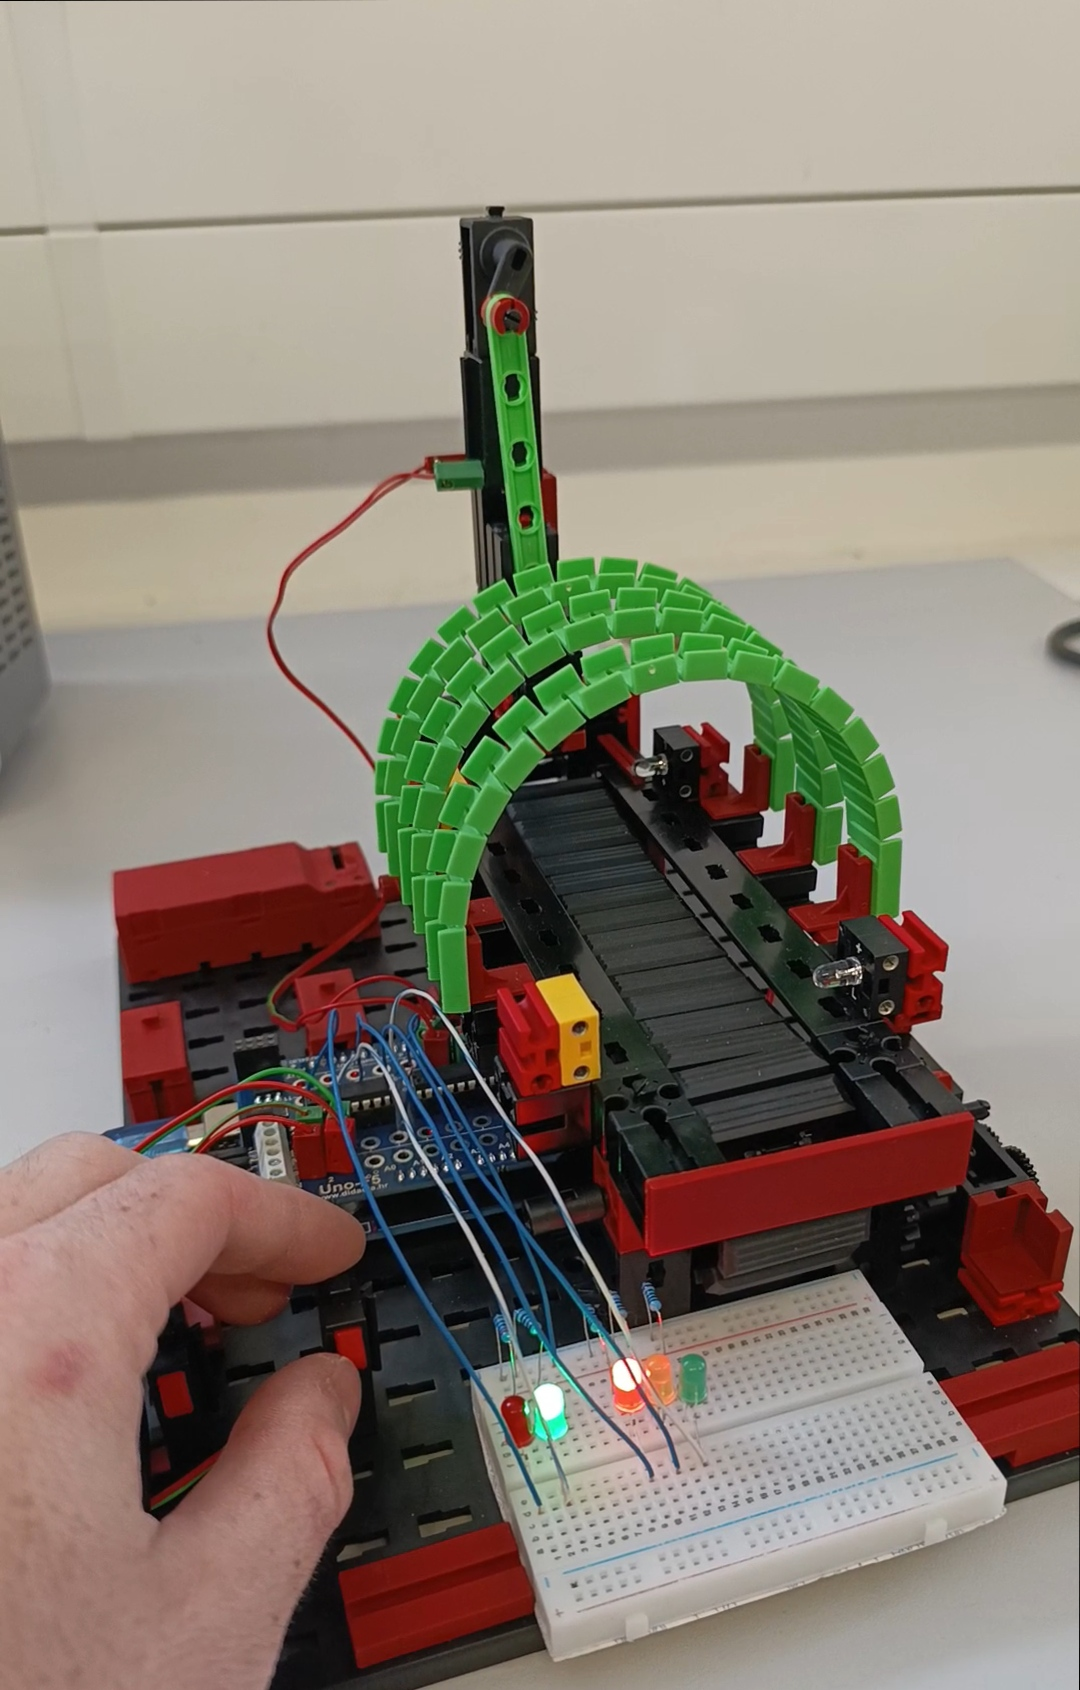
\includegraphics[width=0.7\linewidth]{./Anexos/Resultados/Punzonadora/Circuito.jpg}
  \caption{Ensamblado final de punzonadora. Fuente: \cite{LabDrive}.}
  \label{fig:punzonadora_circuito}
\end{figure}


\subsection{Plotter}

\subsubsection{Mapeo de comandos}
\begin{verbatim}
.equ SOLENOID_DOWN =	0b00000100
.equ SOLENOID_UP =		0b00001000
.equ DOWN =				0b00010000
.equ UP =				0b00100000
.equ RIGHT =			0b01000000
.equ LEFT =				0b10000000
.equ STOP =				0b00000000
\end{verbatim}
\subsubsection{Interprete de secuencias}
\begin{verbatim}
DRAW:
    mov ZL, r16 mov ZH, r17
    DRAW_LOOP:
    lpm r18, Z+ ; Time
    lpm r19, Z+ ; Instruction

    out PORTD, r19 ; Send instruction

    cpi r19, STOP
    breq DRAW_END ; Stop drawing

    DRAW_TIMER_LOOP: ; Timer
    rcall S1
    dec r18 brne DRAW_TIMER_LOOP 

    rjmp DRAW_LOOP ; Next instruction

    DRAW_END:
    ret
\end{verbatim}
Nota: se encontró que para temporizadores con valores menores a 1ms no permitían el movimiento adecuado de los motores, por lo cual se decidió limitar la resolución con un temporizador de 1500 $\mu S$
El siguiente ejemplo es de un programa hecho para el interprete creado para el plotter:
\begin{verbatim}
TRIANGLE_DATA:
    .db 5, SOLENOID_DOWN	
    .db 20, SOLENOID_DOWN + RIGHT			
    .db 10, SOLENOID_DOWN + UP + LEFT		
    .db 10, SOLENOID_DOWN + DOWN + LEFT
    .db 5, SOLENOID_UP		
    .db 5, STOP
\end{verbatim}

\subsubsection{USART}
Ejemplo de caso de interrupción de USART para dibujado de circulo:
\begin{verbatim}
; ...
USART_RX_ISR_CASE_5: ; CIRCLE
    ldi r16, low(CIRCLE_DATA<<1) 
    ldi r17, high(CIRCLE_DATA<<1)
    rcall DRAW
    rjmp USART_RX_ISR_END
\end{verbatim}

\begin{figure}[H]
  \centering
  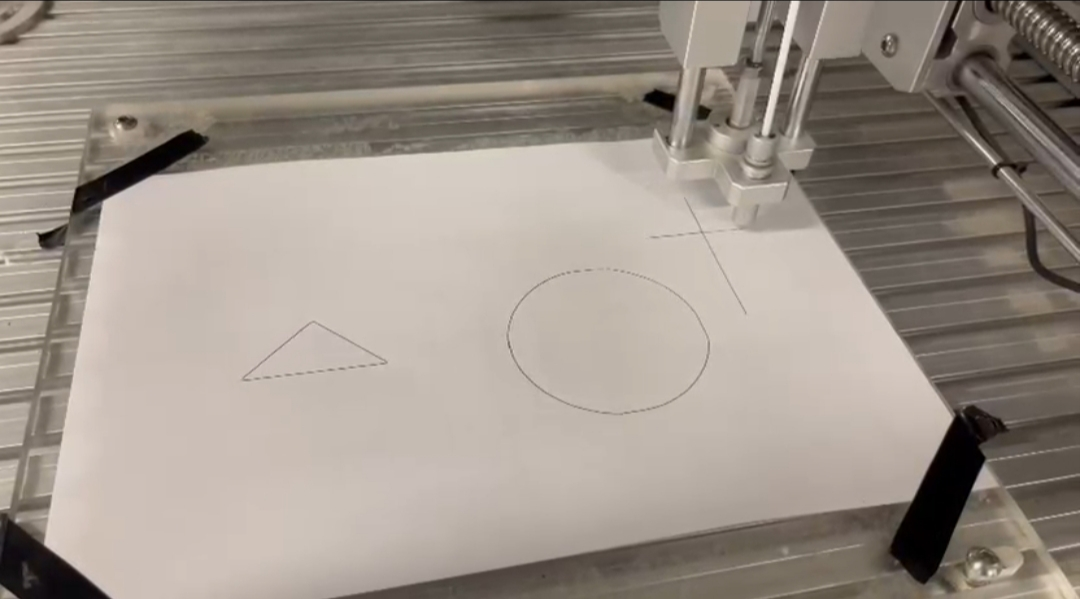
\includegraphics[width=\linewidth]{./Anexos/Resultados/Plotter/Dibujos.jpg}
  \caption{Figuras dibujadas en el plotter. Fuente: \cite{LabDrive}.}
  \label{fig:plotter_figuras}
\end{figure}